\section{Model}
\label{sec:model}

\subsection{Definition}

Each site $i$ of an $L_x\times L_y$ square lattice with periodic boundaries carries a state
$\sigma_i\in\{0,1\}$. Let $j_i$ be the number of sites among the eight Moore neighbors of $i$
whose state differs from $\sigma_i$. In one time step every site is updated simultaneously and
flips with probability $w(j_i)$, independently of the others, where
\begin{equation}
w(j) = (1-p)\,\alpha\,R(j) + p\,\frac{j}{8} + q\,\delta_{j,2},
\label{eq:rule}
\end{equation}
with $R(j) = 1$ for $j\in\{3,6,7,8\}$ and $R(j) = 0$ otherwise. The first term is the D\&N rule
B3678/S34678: a dead site becomes alive if it has 3, 6, 7, or 8
live neighbors, and a live site survives if it has 3, 4, 6, 7, or 8. The rule is
self-complementary, so in terms of disagreeing neighbors a site flips if and only if
$j\in\{3,6,7,8\}$, whatever its state. With probability $\alpha$ a site applies this flip
($\alpha$-asynchronous updating~\cite{fates2005,blok1999}). The second term is the synchronous
voter model on the Moore neighborhood: with probability $p$ the site copies a randomly chosen
neighbor. Since $w$ depends on the configuration only through $j$, Eq.~\eqref{eq:rule} is a
synchronous nonlinear voter model~\cite{cox1991,molofsky1999,schweitzer2009} with a nonmonotone
rate. The third term is a minority flip: a site with exactly two disagreeing neighbors flips
with additional probability $q$. We fix $\alpha = 1/2$ unless stated otherwise and use $q$ as the
control parameter; $p$ interpolates between the D\&N and voter contributions.
The voter point itself is $(p,q)=(1,0)$.
The probability range is $0\le p,\alpha\le1$ and $0\le q\le1-p/4$;
all simulated points lie within it.

Since $w(0) = 0$, the uniform states (all 0, all 1) are absorbing, and Eq.~\eqref{eq:rule} is
invariant under $\sigma\to 1-\sigma$. At $p=\alpha=1/2$, the sampled lower-$q$ runs coarsen toward the
absorbing states. Larger-$q$ runs sustain a disordered active region with
finite interface density and magnetization near zero over the observed windows.

\begin{figure*}
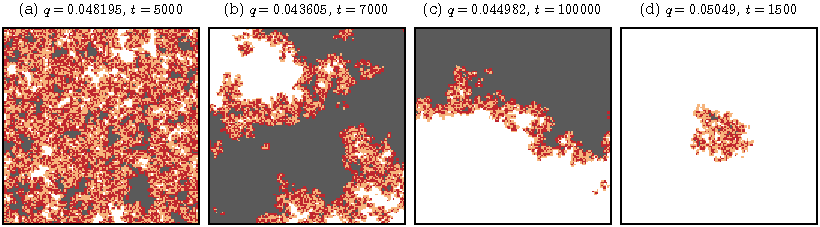
\includegraphics[width=\textwidth]{figs/fig_snap}
\caption{Configurations at $p = \alpha = 1/2$. Sites without a disagreeing Moore
neighbor are white (dead) or gray (alive); sites with at least one are orange (dead) or red
(alive). (a) The active phase, $q = 0.048195$, $t = 5000$, $L = 256$. (b) Decay of the metastable
active phase by nucleation and growth of the two absorbing phases, $q = 0.043605$, $t = 7000$
($256^2$ window of $L = 512$). (c) A wall between the two absorbing phases, wetted by a layer of the
active phase, $q = 0.044982$, $t = 10^5$. (d) A supercritical droplet, $q = 0.05049$, $t = 1500$,
grown from a disordered disk of radius 20.}
\label{fig:snap}
\end{figure*}

\subsection{Exactly two absorbing states}
\label{sec:lemma}

A configuration is absorbing when no site can flip, i.e., when $w(j_i) = 0$ for all $i$.

\textit{Lemma.} On the square lattice with the Moore neighborhood, every rule with $w(0)=0$ and $w(j)>0$ for
all $j\in\{3,\dots,8\}$ has exactly two absorbing configurations, the two uniform ones,
whatever the values of $w(1)$ and $w(2)$.

\textit{Proof.} A nonuniform configuration contains two nearest neighbors $x$ and $y$ (sharing an
edge) in different states. They disagree with each other, and they share four further Moore
neighbors, each of which disagrees with exactly one of them. Hence $j_x + j_y \ge 2 + 4 = 6$, so
$j_x\ge 3$ or $j_y\ge 3$, and that site flips with positive probability. $\square$

For $p>0$, Eq.~\eqref{eq:rule} gives $w(j)\ge pj/8>0$ for every $j\ge 1$, so the lemma applies.
For $0<p<1$ and $0<\alpha<1$ in the parameter range studied, $w(j)<1$ as well. Every configuration of a finite lattice then reaches consensus with
positive probability (by repeatedly flipping only the boundary sites of the live clusters), so
the two uniform states are the only recurrent ones.
At $p=0$, additional frozen configurations exist in exponentially large
number (Supplemental Sec.~\ref{S-app:frozen}); that directly simulated reference
lies outside the exactly-two-state regime. The representative point below
is nonmonotone; the conditions for attractiveness and the pair approximation
are given in Supplemental Secs.~\ref{S-sec:mf} and \ref{S-app:pa}.

\subsection{Observables}

We measure the density $\rho$ of disagreeing nearest-neighbor bonds (the interface density per
bond), the fraction $\iota$ of sites with at least one disagreeing Moore neighbor, and the
magnetization $m = 2n-1$, where $n$ is the fraction of live sites. In the active phase
$\rho\approx 0.2$--$0.4$ and $m$ fluctuates around zero; in either uniform
absorbing phase $\rho = \iota = 0$.
The bond density is our activity order parameter. If $a$ denotes the expected
fraction of sites flipping in one step, then
\begin{equation}
 a=\frac{1}{L^2}\sum_i w(j_i)\ge\frac{p}{8L^2}\sum_i j_i\ge\frac{p}{2}\rho .
 \label{eq:activitybound}
\end{equation}
The last inequality counts just the four axial neighbors. Thus, for $p>0$,
a positive bond density implies positive microscopic flip activity.

Since every finite lattice ultimately absorbs at the interior parameters,
the active branch refers to the order of limits
\begin{equation}
 \rho_{\rm act}(q)=\lim_{t\to\infty}\lim_{L\to\infty}
     \mathbb E_{1/2}[\rho_L(t;q)],
 \label{eq:limits}
\end{equation}
when this limit exists, starting from independent density-$1/2$ spins.
A discontinuity means a positive active-side limit on approaching a phase
boundary $q_c$. Our measurements are finite-volume, finite-time diagnostics
of that property. We denote a measured front crossing by $q^*$, with its
window and geometry stated; it need not be a unique limiting $q_c$.
At generalized voter criticality $\rho$ vanishes logarithmically, while a
magnetization jump can still occur~\cite{dornic2001,alhammal2005}.
We therefore compare density with coherent front reversal, metastable decay,
and the response to prepared droplets.

Spatial correlations use $s_i=2\sigma_i-1$ and the axis average
\begin{equation}
C(r)=\frac{1}{2L^2}\left\langle\sum_i s_i
\bigl(s_{i+r\hat x}+s_{i+r\hat y}\bigr)\right\rangle.
\label{eq:correlation}
\end{equation}
The random-start ensemble is exactly spin symmetric, so $\langle s_i\rangle=0$.
We retain the raw spin product, including $C(r)=1$ in absorbed configurations,
and do not subtract a separately estimated mean from each realization.

%=====================================================================================
